\chapter{Os Métodos de Análise}
\label{chapter:os_metodos_de_analise}

\section{\textbf{K-nearest Neighbors}}

Existem vários métodos de análise de algoritmos, um dos mais simples é o “K-Nearest Neighbors”, utilizado no Script, que funciona da seguinte forma:

Observando a imagem abaixo, observa-se um gráfico com um conjunto de bolas amarelas e roxas; também é possível perceber uma bola desconhecida, destacada na cor vermelha. Para calcular se ela é roxa ou amarela, o algoritmo do KNN determinará a sua cor, de acordo com as N bolas mais próximas.

Por exemplo, caso N seja igual a 3, a bola desconhecida será classificada como roxa e no caso de N igual à 6 será classificada como amarela:

\begin{figure}[!htb]
\begin{center}
\caption{K-nearest Neighbors}
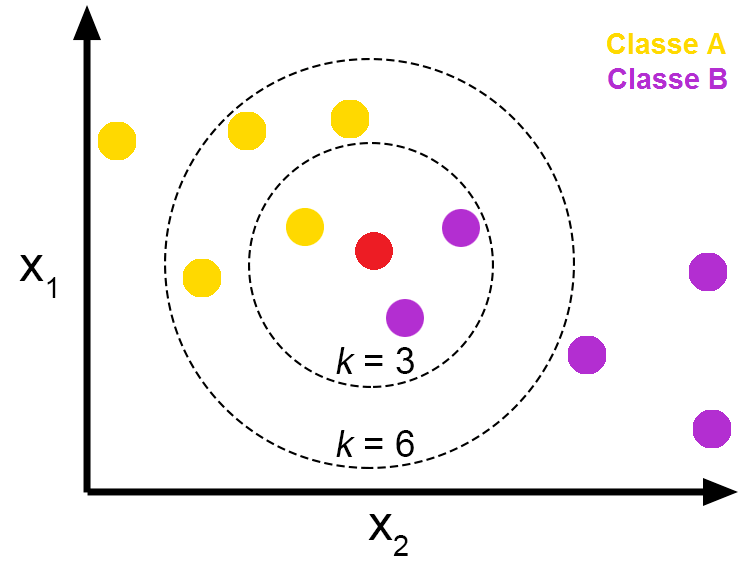
\includegraphics[width=8cm]{knearestneighbors}
\end{center}
\legend{Fonte: https://miro.medium.com/max/1506/0*jqxx3-dJqFjXD6FA}
\cite{KNN}
\end{figure}




\section{\textbf{Decision tree}}

A chamada “Árvore de Decisão”, define um novo elemento com base em rotinas pré-estabelecidas. Por exemplo, se há um banco de dados de pessoas que foram jogar tênis com base na situação do clima, pode-se chegar a seguinte árvore de decisão:


\begin{figure}[!htb]
\begin{center}
\caption{Decision Tree}
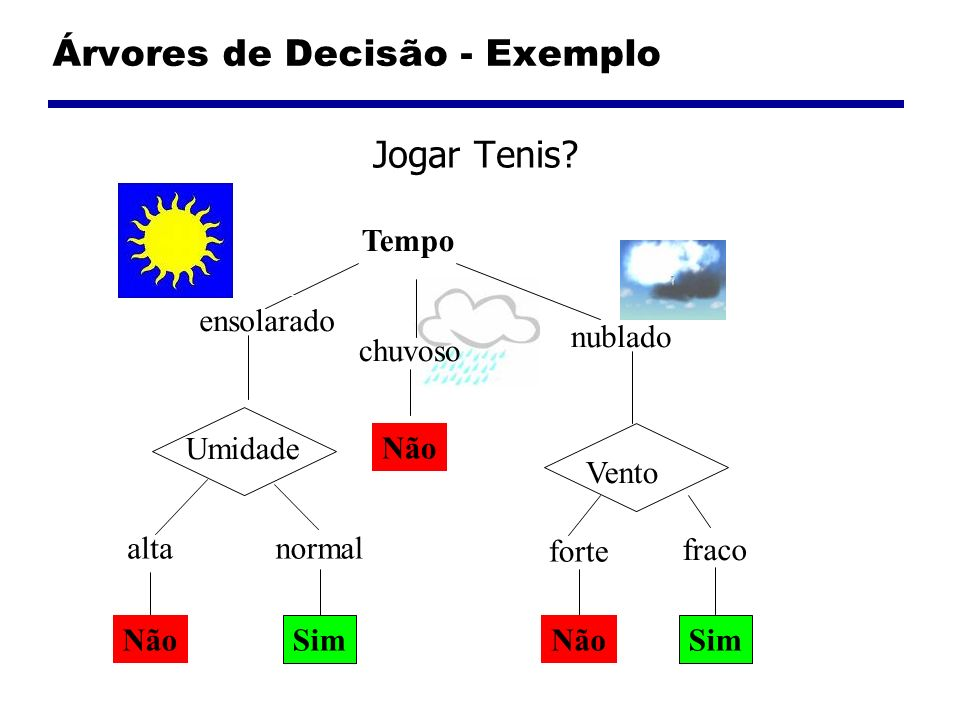
\includegraphics[width=8cm]{decisiontree}
\end{center}
\legend{Fonte: https://slideplayer.com.br/slide/358847/2/images/5/\%C3\%81rvores+de+Decis\%C3\%A3o+-+Exemplo.jpg}
\cite{ARVOREDECISAO}
\end{figure}

E então quando alguém perguntar se haverá jogo de tênis no dia, ela responderá de acordo com o clima, seguindo a árvore de decisão.

\section{\textbf{Random Forest}}

Algoritmo que cria várias árvores de decisões, definido anteriormente, e as combinam para obter uma predição com maior acurácia e mais estável:



\begin{figure}[!htb]
\begin{center}
\caption{Random Forest}
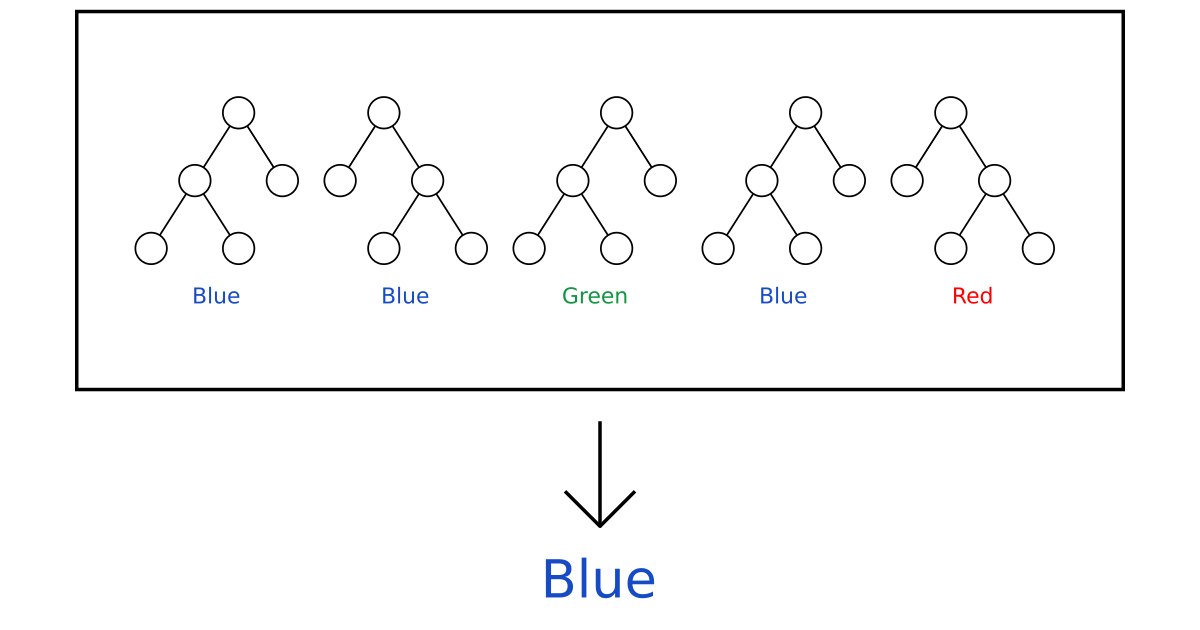
\includegraphics[width=8cm]{randomforest}
\end{center}
\legend{Fonte: https://victorzhou.com/media/random-forest-post/random-forest.png}
\cite{RANDOMFOREST}
\end{figure}



\section{\textbf{Support Vector machine}}

O classificador intitulado de “Máquina de Vetores de Suporte” categoriza, com base em uma divisão dos dados.  

Por exemplo, na imagem abaixo, há quadrados e círculos de cores vermelhas e azuis, respectivamente. 
Pode-se dividi-las com qualquer uma das retas do quadrante esquerdo. 
Porém, como mostrado no quadrante direito, 
há uma única reta em que a sua distância em relação a figura azul mais próxima é igual a distância da figura vermelha mais próxima, 
logo se encontra a melhor reta para separá-las.


\begin{figure}[!htb]
\begin{center}
\caption{Suport Vector Machine}
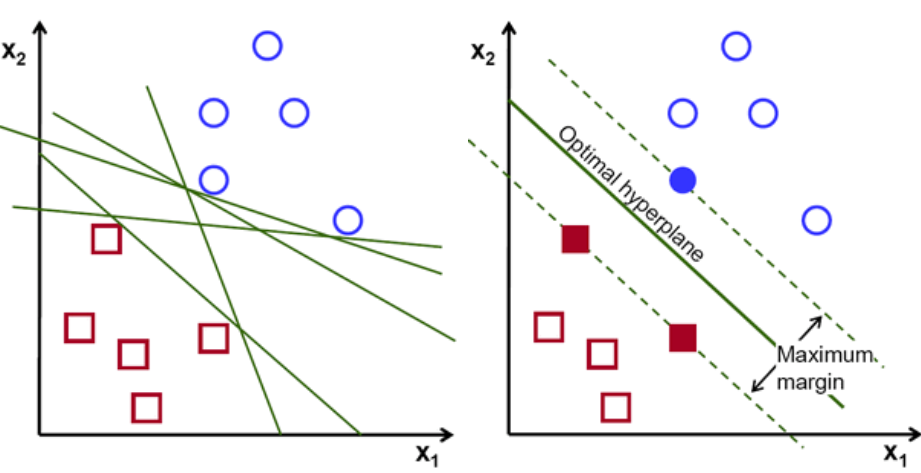
\includegraphics[width=8cm]{suportvectormachine}
\end{center}
\legend{Fonte: https://miro.medium.com/max/921/1*nUpw5agP-Vefm4Uinteq-A.png}
\cite{SVM}
\end{figure}

Em casos mais complexos utilizam-se hiperplanos.


\section{\textbf{Naive bayes}}

O classificador “Naive Bayes” é baseado no Teorema de Bayes. Ele desconsidera a correlação entre as variáveis, e por isso é chamado de “ingênuo”. 

Um exemplo de sua utilização seria para considerar se um fruto qualquer é uma maçã, assim, analisa-se se ele é vermelho, redondo e de aproximadamente 3 polegadas (Características da fruta colocada em exemplo). De acordo com o Teorema de Bayes, cada um desses fatores contribui independentemente para a probabilidade de que este fruto seja realmente uma maçã.

Quando se lida com muitos dados, sendo eles todos independentes, assumisse que distribuição ocorre de acordo com uma gaussiana simples, por isso usa-se o classificador GauissanNB para calculá-lo.


\begin{figure}[!htb]
\begin{center}
\caption{Naive Bayes}
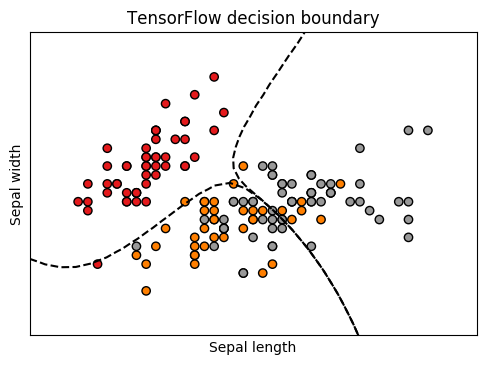
\includegraphics[width=8cm]{naivebayes}
\end{center}
\legend{Fonte: https://nicolovaligi.com/tf\_iris.png}
\cite{NAIVEBAYES}
\end{figure}


\section{\textbf{Artificial Neural Network}}

A chamada, “Rede neural artificial” é um classificador que se baseia no sistema de redes neurais que utiliza o mecanismo de aprendizagem de pesos sinápticos de tal forma que a unidade de saída produza as respostas corretas para cada exemplo, realizando atualizações de forma dinâmica e interativa até chegar aos pesos corretos.

É a mais parecida, com o sistema que ocorre no cérebro:


\begin{figure}[!htb]
\begin{center}
\caption{Artificial Neural Network}
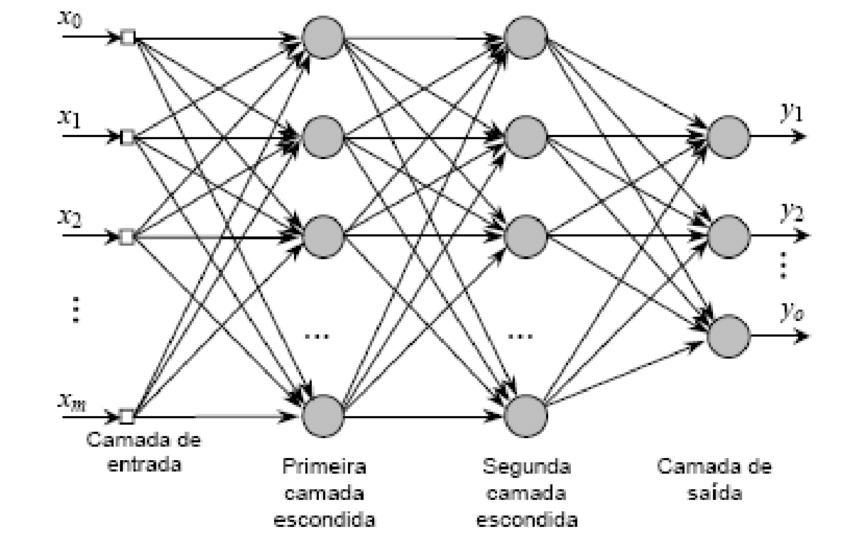
\includegraphics[width=8cm]{mlp}
\end{center}
\legend{Fonte: https://www.researchgate.net/profile/Anderson\_Oliveira6/publication/240772105/figure/fig2/AS:667857415319554@1536241024122/Figura-1-Rede-Neural-Artificial-Multicamadas.png}
\cite{MLP}
\end{figure}


